\subsection{Complejidad}

Para encontrar la complejidad de nuestra solución, tenemos que analizar dos algoritmos, uno recursivo y el otro que busca el master, ambos con sus respectivos pseudocódigos detallados en el punto anterior.

En ambos algoritmos, tenemos un arreglo de nodos 'arbol', acceder a uno de ellos con un índice me cuesta O(1).

En el primero tenemos un ciclo, y dentro de él un llamado recursivo. El algoritmo no vuelve a pasar por un nodo en el que estuvo, es decir arribo a cada nodo por exactamente una de las aristas y luego me muevo hacia las demás. De esta manera encuentro una cota para la cantidad de llamados recursivos, que es n el número de nodos.

En un llamado a la función, el ciclo realiza una cantidad de iteraciones igual a la cantidad de nodos adyacentes y realiza un llamado en todos excepto aquel por el que vino. Esto significa que en toda la ejecución, cada arista es atravesada por dos nodos (pero el llamado recursivo se hace en uno de los dos), y como el número de aristas es n-1, puedo decir que el número de iteraciones del ciclo en toda la ejecución está acotado por 2n. 

\begin{center}
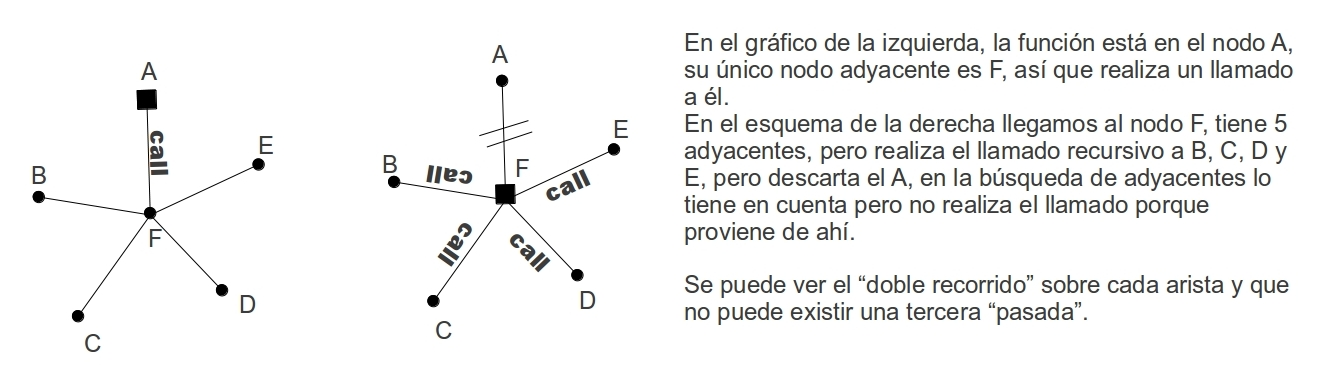
\includegraphics[scale=0.5]{ej2/2/graficos/imagen04.jpg} 
\end{center}

De esta manera puedo afirmar que el ciclo itera a lo sumo 2n veces, y lo que está fuera de él n veces (En total durante toda la ejecución)


\underline{Análisis del algoritmo recursivo}:

\textbf{Línea 2}: Preguntar si quedan "hijos" es decir nodos adyacentes, es \textbf{constante} ya que tengo un arreglo Arbol y el índice en el arreglo que cuesta O(1) acceder y luego empiezo a recorrer la lista con los adyacentes.

\textbf{Línea 3}: Tomo cualquiera de los hijos de la lista, es \textbf{constante}.

\textbf{Líneas 4 y 5}: Acá se hace el llamado recursivo, tiene complejidad \textbf{constante} hacer el llamado, ya tengo acotada la cantidad de llamados así que solamente hago el análisis de las operaciones que empleo en la función. El if también es de complejidad \textbf{constante}.

\textbf{Línea 6}: La función que uso en esta línea realiza un par de comparaciones para determinar los dos valores mayores de los tres que recibe. Complejidad \textbf{constante}.

\textbf{Línea 8}: Fin del ciclo, ya tengo acotada la cantidad de iteraciones totales (suma de iteraciones entre todos los llamados) así que el análisis de iteraciones lo dejo para después por ahora sólo digo que tengo una suma de complejidades constantes, así que la complejidad del ciclo (sin tener en cuenta iteraciones) es\textbf{ constante}.

\textbf{Líneas 9 y 10}: Actualiza la información del nodo en el arreglo con los valores definitivos, y devuelve un valor. También complejidad \textbf{constante}.

Por un lado tengo que la cantidad de llamados a la función durante toda la ejecución está acotada por n, entonces las líneas 9 y 10 se ejecutan a lo sumo n veces, es decir que tenemos O(1) x n = O(n).
Además sé que el ciclo que tiene complejidad constante para una iteración, durante toda la ejecución itera a lo sumo 2n veces, obtenemos O(1) x 2n = O(2n).


De esta manera para calcular la complejidad del algoritmo en una ejecución, debo sumar las complejidades de ambos. O(n) + O(2n) = O(3n) = O(n)

Nos queda ver la complejidad del segundo algoritmo, se ejecuta una única vez, por lo tanto con la suma de las complejidades de cada una de sus operaciones, voy a obtener la complejidad total del algoritmo, que luego sumada a la complejidad que calculé para el algoritmo 1, obtengo cual es la complejidad de mi resolución del problema.

\underline{Análisis del Algoritmo 2, para encontrar el master:}

\textbf{Línea 1}: Recorre el arreglo 'arbol' buscando el elemento que posee el mayor campo suma. A lo sumo recorro todo el arreglo por lo tanto tengo una complejidad en el orden \textbf{O(n)}.

\textbf{Líneas 2 y 3}: Obtengo valores del arreglo, accediendo con un índice. Complejidad \textbf{constante}.

\textbf{Línea 4}: Tenemos un ciclo que itera una cantidad de veces igual a la mitad de la longitud del máximo camino en un árbol. Un camino máximo puede ser de a lo sumo n-1 aristas, así que puedo acotar el número de iteraciones en n veces.

\textbf{Línea 5}: Acceso a un campo de un elemento del arreglo, con un determinado índice. Complejidad \textbf{constante}.

\textbf{Líneas 6 y 7}: Sumo y resto valores, complejidad \textbf{constante}.

Entonces tenemos un ciclo que itera n veces, dentro del cual hay operaciones de complejidad constante, ésto es O(1) x n = O(n). Y en la línea 1 teníamos un recorrido por el arreglo en el orden de O(n), por lo tanto este algoritmo tiene una complejidad de O(n) + O(n) = O(2n).

\underline{Complejidad total} (algoritmo 1 + algoritmo 2):
Ahora ya tengo las complejidades de ambos, las sumo y obtengo el total:
O(n) + O(n) = O(2n) = O(n)

Queda demostrado que nuestra solución se encuentra dentro de la complejidad exigida por el enunciado.  